\documentclass[letterpaper]{article}
\usepackage{natbib,alifeconf}
\usepackage{hyperref}


\usepackage[flushleft]{threeparttable}
\usepackage{subcaption}
\usepackage{booktabs}
\setcounter{tocdepth}{3}
\usepackage{array}
\usepackage{float}
\usepackage{dirtytalk}


\title{Evolution of Heterogeneous Cellular Automata in Fluctuating Environments}
\author{First Author$^{1}$, Second Author$^{1,2}$, Third Author$^{1,2}$, Fourth Author$^{1,2}$ \and Fifth Author$^2$ \\
\mbox{}\\
$^1$First affiliation  \\
$^2$Second affiliation \\
corresponding@author.email}


\begin{document}
\maketitle

\begin{abstract}
The importance of environmental fluctuations in the evolution by natural selection of living beings has been widely noted by biologists and such fluctuations have been linked to many important characteristics of life such as: modularity, plasticity, genotype size, mutation rate, and learning or epigenetic adaptations. However, in artificial life simulations, environmental fluctuations are usually seen as a problem to be solved rather than an essential characteristic of evolution. We propose in this paper to use HetCA to measure the impact of different forms of environmental fluctuations, where HetCA is a heterogeneous cellular automata characterized by its ability to generate open ended long-term evolution and evolutionary progress, Our results indicate that environmental fluctuations induce mechanisms analogous to epigenetic adaptations in HetCA.
\end{abstract}



\section{Introduction}
Environmental changes may include cyclic events such as seasonal changes or a daily cycle of light and darkness, occasional changes such as the introduction of new predator or the potential for a new source of food, or much more radical modifications to the environment such as environmental stress induced by climate change.

Early population genetics theory assumed the environment to be constant. However, since then, work such as that of Richard Levins~\cite{levins1968evolution} in the 70's and more recently Eva Jablonka et al.~\cite{jablonka2014evolution}, the importance of environmental fluctuations in the evolution by natural selection of living beings has been widely noted. Through these and other works, environmental fluctuations have been linked to many important questions about the mechanisms of evolution such as: modularity, plasticity	~\cite{west2005developmental}, size of the genotype, mutation rate and evolvability. In Jablonka et al.~\cite{jablonka2014evolution} stresses that a changeable environment will unmask variations in the capacity of individuals to make adjustments to changed conditions and therefore promote plasticity. They are also taking into account the idea that \say{For a lineage in a constantly changing environment, switching among several alternative heritable states was probably an advantage. While cells in one state survived in one set of conditions, those in other states did better in other states did beter in other set of circumstances.} and hypothesize that constantly changing environment or cycling variations might explain the origin of the Epigenetic Inheritance Systems, considering epigenetic mutations are more reversibles and occure more frequently than genetic mutations. 

In \cite{lachmann1996inheritance} Lachemann modelled the effects of cycling variations, such as seasonal or daily cycles, on phenotypical inheritances. Their model predicted that when the investigated cycles are longer than the reproductive cycle but relatively short otherwise, heritable variations produced by non-DNA inheritance systems are likely to be observed.

A proportion of existing work in artificial life, especially in evolutionary robotics\cite{floreano2000evolutionary}, considers the issue of environmental variations. However, it is probably fair to say that, a significant majority of these previous work has either focused on aspects such as normal spatial variation, or has viewed environmental change as a problem to be solved.

This paper is organized as follows. Section~\ref{sec:bground}, we explain the mechanisms of HetCA simulation. The implementation of environmental fluctuation in HetCA is then explained in Section~\ref{sec:exsetup}. Section 5 details the computer experimental setup while we reports experimental results in Section~\ref{sec:results}. We discuss the implications of these results in Section~\ref{sec:discuss}. Finally, Section~\ref{sec:conc} concludes the paper.


\section{Background}\label{sec:bground}
In~\cite{lipson2002origin} Lipson demonstrated a correlation between the modularity and the rate of change of the environment resources. While in \cite{yu2007program} Yu used observed that populations exploit neutrality to cope with environmental fluctuations and therefore evolve some sort of evolvability under two alternating objective functions. Both of these simulations used Genetic Programming~(GP) and employed explicit fitness functions.

\section{HetCA}\label{sec:hetca)}
HetCA is based on classical two-dimensional cellular automata~(CA), but has several added features: cells have \emph{age}, \emph{decay} and \emph{quiescence} properties; cells utilize a heterogeneous transition function inspired by linear genetic programming~(LGP); and there exists a notion of genetic transfer of transition functions between adjacent cells.

HetCA exhibits long term phenotypic dynamics, sustains a high level of variance over very long runs and displays greater behavioural diversity than classical cellular automata\cite{medernach2013long}. HetCA also exhibits Evolutionary Progress (EP) according to the three criteria : robustness, size and density of generated genotypes\cite{medernach2015evolutionary}, using Shanahan's definition of EP \cite{shanahan2012evolutionary}.

Moreover, some emergent properties of HECA are similar to two of the five major eukaryotic innovations which do not appear to have direct prokaryotic predecessors defined in~\cite{smith1997major} as : the eukaryotic chromatin remodelling machinery; the cell cycle regulation systems; the nuclear envelope, the cytoskeleton; and the apoptosis apparatus\cite{koonin2002origin}. Indeed, in HetCA, the loss of the genotype of the cell as it turns to the quiescent state may seem similar to apoptosis while survival strategies such as the ones depicted in Figure~\ref{foursteps} might akin cell cycle regulation systems. HetCA intéressant car permet sélection multilevel ref : http://faculty.virginia.edu/vaformica/MLS/images/okasha-Chapters1-2.pdf


\section{Experimental Setup}\label{sec:exsetup}
\subsection{Environmental Fluctuations}
Originally, in HetCA, the new genotype of a cell was randomly chosen among candidate genotypes. In order to introduce environmental variations, we chose to vary the likelihood of spread of the genotype of a cell according to the state of this cell. The chances of the candidate genotype of the cell $c$ to be selected are then: $c=K(S_c)/\sum_{i=1}^{n} K(S_{c_i})$ with $S_c$ state of the cell $c$, $K(S)$ likelihood of spread of state $S$ and $n$ number of candidate genotypes. Therefore an environment is characterized by the odds of propagation of the five living states $\{K(S_1),K(S_2),K(S_3),K(S_4),K(S_5)\}$.   
To mimic environmental fluctuations we initialise the simulation with $K(S_i)=1  \forall i \in [1,5]$ and then we regularly change those values from iteration 3000 of the cellular automata. 

We chose to introduce four forms of environmental fluctuations described in Table~\ref{tab:environments}.

\noindent \emph{Short-cycle Fluctuation}: consists of alternating between two environments every 100 iterations of the cellular automaton. We chose to vary the environment every 100 iterations to stay in the same range of frequency as described in Lispson~\cite{lipson2002origin} examples 20 and 100 generations and~\cite{yu2007program} experiments 10, 20 and 50 generations. In fact we consider that a successful reproductive cycle involves passing a cell through the quiescent state. And this should take between two iterations (alternating between the quiescent state and a living state) and seven iterations (if a cell remains in a living state more than seven consecutive iterations it goes to the decay state and can not receive a genotype for an important period).

\noindent \emph{Light Fluctuation}: consists of alternating between five environments every 5000 iterations of the cellular automaton. The first five each prohibit a different state from the five living state, the latter gives equal chance to each of the five states.

\noindent \emph{Strong Fluctuation}: consists of alternating between twelve environments every 5000 iterations of the cellular automaton. The first eleven each prohibit a different combination of two states from the five living states, the latter gives equal chance to each of the five states.

\noindent \emph{Gradual Fluctuation}: is similar to strong fluctuation except that it includes a transition phase of $T=60$ iterations in between two environments where likelihood of spread of state values progressively switch from the value a previous environment to the ones of the new environment. Over this phase the state spreading is defined by the following formula : $K(S,t)=K_p(S) \times (T-t) + K_{p+1}(S) \times t$ where $t$ is the number of iterations completed since the beginning of the transition phase; $K_p(S)$ and $K_{p+1}(S)$ are likelihood of state spread $S$ for the current environment and the next environment respectively.

\emph{Short-cycle fluctuation} may be analogous to the circadian rhythms for some bacteria: very regular cycles in which these organisms have enough time to reproduce several times. While \emph{light fluctuation} may be similar to seasonal fluctuations and \emph{strong and gradual fluctuations} would akin ecological crisis. Although, owing to the variety of both biological temporal rhythms and reproductive cycles, the relevance of these analogies may be limited. 

\subsection{Common Settings}\label{sec:commonset}
For each form of environmental fluctuation and the stable non fluctuating environment, we performed 50 simulations, each on 500000 iterations with the parameters listed in Table~\ref{settings}. The genotypes of an individual are its transition rules encoded with CA-LGP using the function set depicted in Table~\ref{funcSet}. Mutation of genotypes is enabled and we use the Micro/Marco-mutation of CA-LGP as described in \cite{medernach2013long}.

\begin{table}
\scriptsize
\centering
\begin{tabular}{l>{\centering}p{0.2\columnwidth}}\toprule%
Parameter & Value \tabularnewline
\toprule%
Number of living states & 5\tabularnewline
Successive living iterations before decay & 7\tabularnewline
Number of iterations for decay & 375-1875\tabularnewline
Direct transition to decay & enabled\tabularnewline
Size of the grid & 500x500\tabularnewline
Grid boundaries & toric grid\tabularnewline
Transition Rule~(TR) & CA-LGP\tabularnewline
Maximum (TR) size & 50 program statements\tabularnewline
Genotype copy neighbouring  & Von Neumann \tabularnewline
Transition rule neighbouring & Moore\tabularnewline
\bottomrule%
\end{tabular}
\caption{ \textbf{HetCA parameters}.}
  \label{settings}
\end{table}


\begin{table}
\scriptsize
\centering
  \begin{tabular}{l>{\centering}p{0.6\columnwidth}}
  \toprule%
    \textbf{op. name}	& \textbf{action} on inputs $(x,y)$\tabularnewline
 \toprule%   
    abs			& $|x|$ \tabularnewline
    plus		& $x+y$ \tabularnewline
    delta		& 1, if $|x-y| < 1/10000$; 0 o.w. \tabularnewline
    dist		& $|x-y|$ \tabularnewline
    inv			& $1-x$ \tabularnewline
    inv2		& safeDiv($1, x$) \tabularnewline
    magPlus		& $|x+y|$ \tabularnewline
    max			& $\max \{x,y\}$ \tabularnewline
    min			& $\min \{x,y\}$ \tabularnewline
    safeDiv		& $x/y$ if $|y| >  1/10000$; 1 o.w. \tabularnewline
    safePow		& $x^y$, if defined; 1 o.w. \tabularnewline
    thresh		& 1, if $x > y$; 0 o.w.\tabularnewline
    times		& $xy$ \tabularnewline
    zero		& 1, if $|x| < 1/10000$; 0 o.w. \tabularnewline
\bottomrule%
  \end{tabular}
    \caption{\textbf{Function set}. \label{funcSet}}
\end{table}

\section{Methodology}\label{sec:method}

\subsection{Genotype Size}
We use the number of program statements ($n_{prog}$) as a measure of the genotype size and compute the average size of all the current genotypes of a run every 2500 iterations. We then report the average and standard error among all the fifty runs sharing the same settings.

\subsection{Changes induced by environmental fluctuation}
To measure the impact of environmental fluctuations on the phenotypes we compare, for each run, their data at iteration $t$ with that at iteration $t + 5000$ ($t + 7500$ for \emph{Short-cycle Fluctuation}).

\subsection{Density}
We also collect the \emph{most common genotype}~(most frequently occurring) in iterations 2500\footnote{\cite{medernach2015evolutionary}  has shown that the most common genotypes during the first iterations of HetCA were unlikely to have a viable survival strategy, therefore we chose to collect genotypes from iteration 2500.}, 102500, 202500, 302500, 402500 and 500000. 

\subsection{Regularities measurement} 
In HetCA, to survive in the long term the genotypes must regularly release cells by transforming them into quiescent cells without genotypes. This generates patterns and cycles which are quite easy to observe in homogeneous simulations where a single genotype is tested as shown in Figure~\ref{foursteps}, but also observable, although with more difficulty, in normal, heterogeneous, HetCA simulations as seen in Figure~\ref{fourstepsreal}. That is why we found it useful to measure these cycles as well as out-of regularities. If the genotype of a cell adopts a stable strategy, i.e. repeats a sequence of states, this sequence must contain a minimum of two states in order to ensure the survival of the genotype -- the quiescent state and one of the living states.  
 
\begin{figure}[h]
\centering
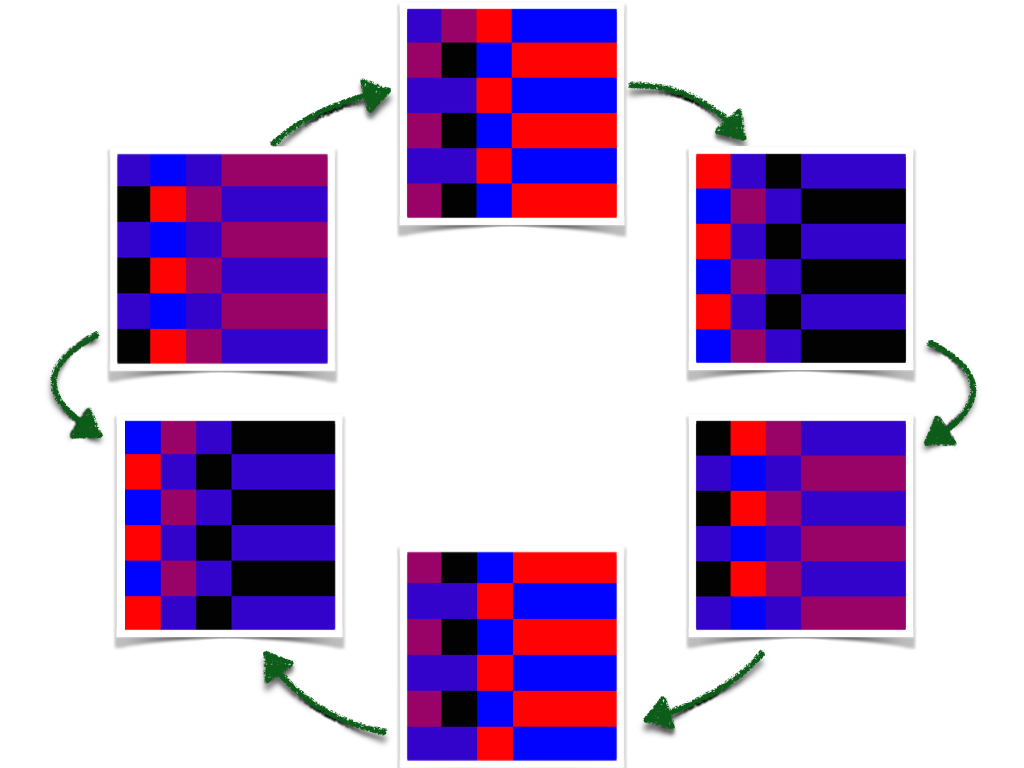
\includegraphics[width=0.75\columnwidth]{4steptransition}
\caption{\textbf{Six steps survival strategy} from a genotype extracted from a HetCA simulation in a stable environment and tested here in a randomly initialized homogenous CA. }
  \label{foursteps}
\end{figure}
 
\begin{figure}[h]
\centering
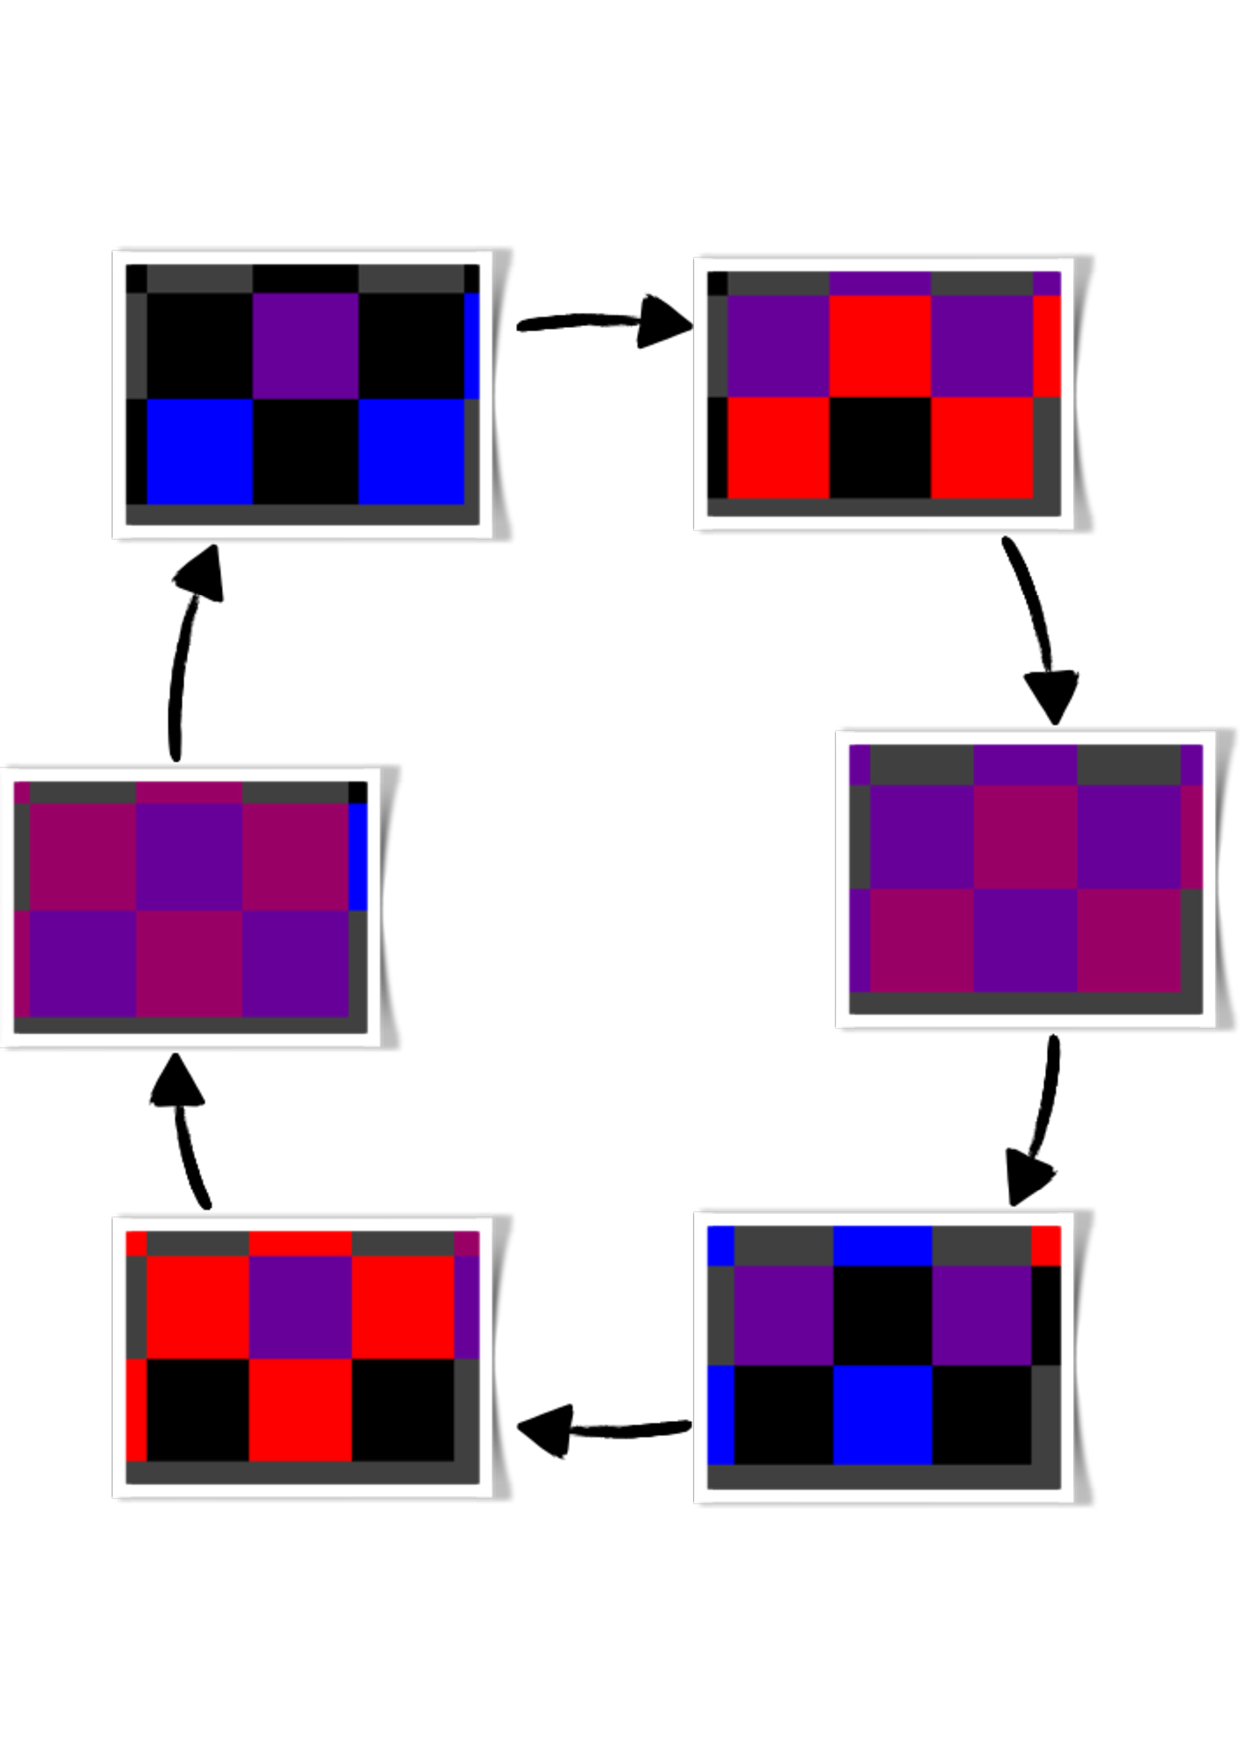
\includegraphics[width=0.75\columnwidth, angle =-90]{cyclesReal}
\caption{\textbf{Six steps survival strategy} from a HetCA simulation with \emph{Short-cycle Fluctuation}. }
  \label{fourstepsreal}
\end{figure}

For this, at every iteration of the genotype density test, we compare the state of each cell to their state during the eight previous iterations of the CA. We then measure whether a sequence of states is repeated during these eight iterations, and if so what is its frequency $f=1/k$ with $\min k \in [2;7], S_t=S_{t-k} \wedge S_{t-1}=S_{t-1-k}$ where $S_t$  is the state of the considered cell at iteration $t$.


\newcommand*{\TitleParbox}[1]{\parbox[l]{10cm}{\raggedright #1}}%
\begin{table*}
\caption{Environments.\label{tab:environments}}
\scriptsize

\begin{tabular}{lccccl}
\toprule%
{\textbf{Name}} & {\textbf{Short Name}} & \textbf{Cycles}\tnote{a} & \textbf{Transitions}\tnote{b} &\textbf{Environment list} \tabularnewline
\toprule%
\textbf{Stable Environment} & [SE] & NA & NA & \TitleParbox{$\{1,1,1,1,1\}$} \tabularnewline

\textbf{Short-cycle Fluctuations} & [ScF] & 100 & 1 & \TitleParbox{$\{1,1,1,0,0\}$, $\{1,1,1,0,0\}$} \tabularnewline

\textbf{Light Fluctuations} & [LF] & 5000 &  1 & \TitleParbox{$\{1,1,1,1,0\}$, $\{1,1,1,0,1\}$, $\{1,1,0,1,1\}$, $\{1,0,1,1,1\}$, $\{0,1,1,1,1\}$, $\{1,1,1,1,1\}$}\tabularnewline
    
\textbf{Strong Fluctuations} & [SF] & 5000 & 1 & \TitleParbox{$\{0,0,1,1,1\}$, $\{1,1,1,0,0\}$, $\{0,1,0,1,1\}$, $\{1,0,1,1,0\}$, $\{0,1,1,0,1\}$, $\{1,1,0,1,0\}$, $\{1,0,1,0,1\}$, $\{0,1,1,1,0\}$, $\{1,0,0,1,1\}$, $\{1,1,0,0,1\}$, $\{1,1,1,1,1\}$} \tabularnewline

\textbf{Gradual Fluctuations} & [GF] & 5000  & 60 & \TitleParbox{$\{0,0,1,1,1\}$, $\{1,1,1,0,0\}$, $\{0,1,0,1,1\}$, $\{1,0,1,1,0\}$, $\{0,1,1,0,1\}$, $\{1,1,0,1,0\}$, $\{1,0,1,0,1\}$, $\{0,1,1,1,0\}$, $\{1,0,0,1,1\}$, $\{1,1,0,0,1\}$, $\{1,1,1,1,1\}$} \tabularnewline

\bottomrule%
\end{tabular}%
\end{table*} 



\section{Results}\label{sec:results}
\begin{figure}[h]
\centering
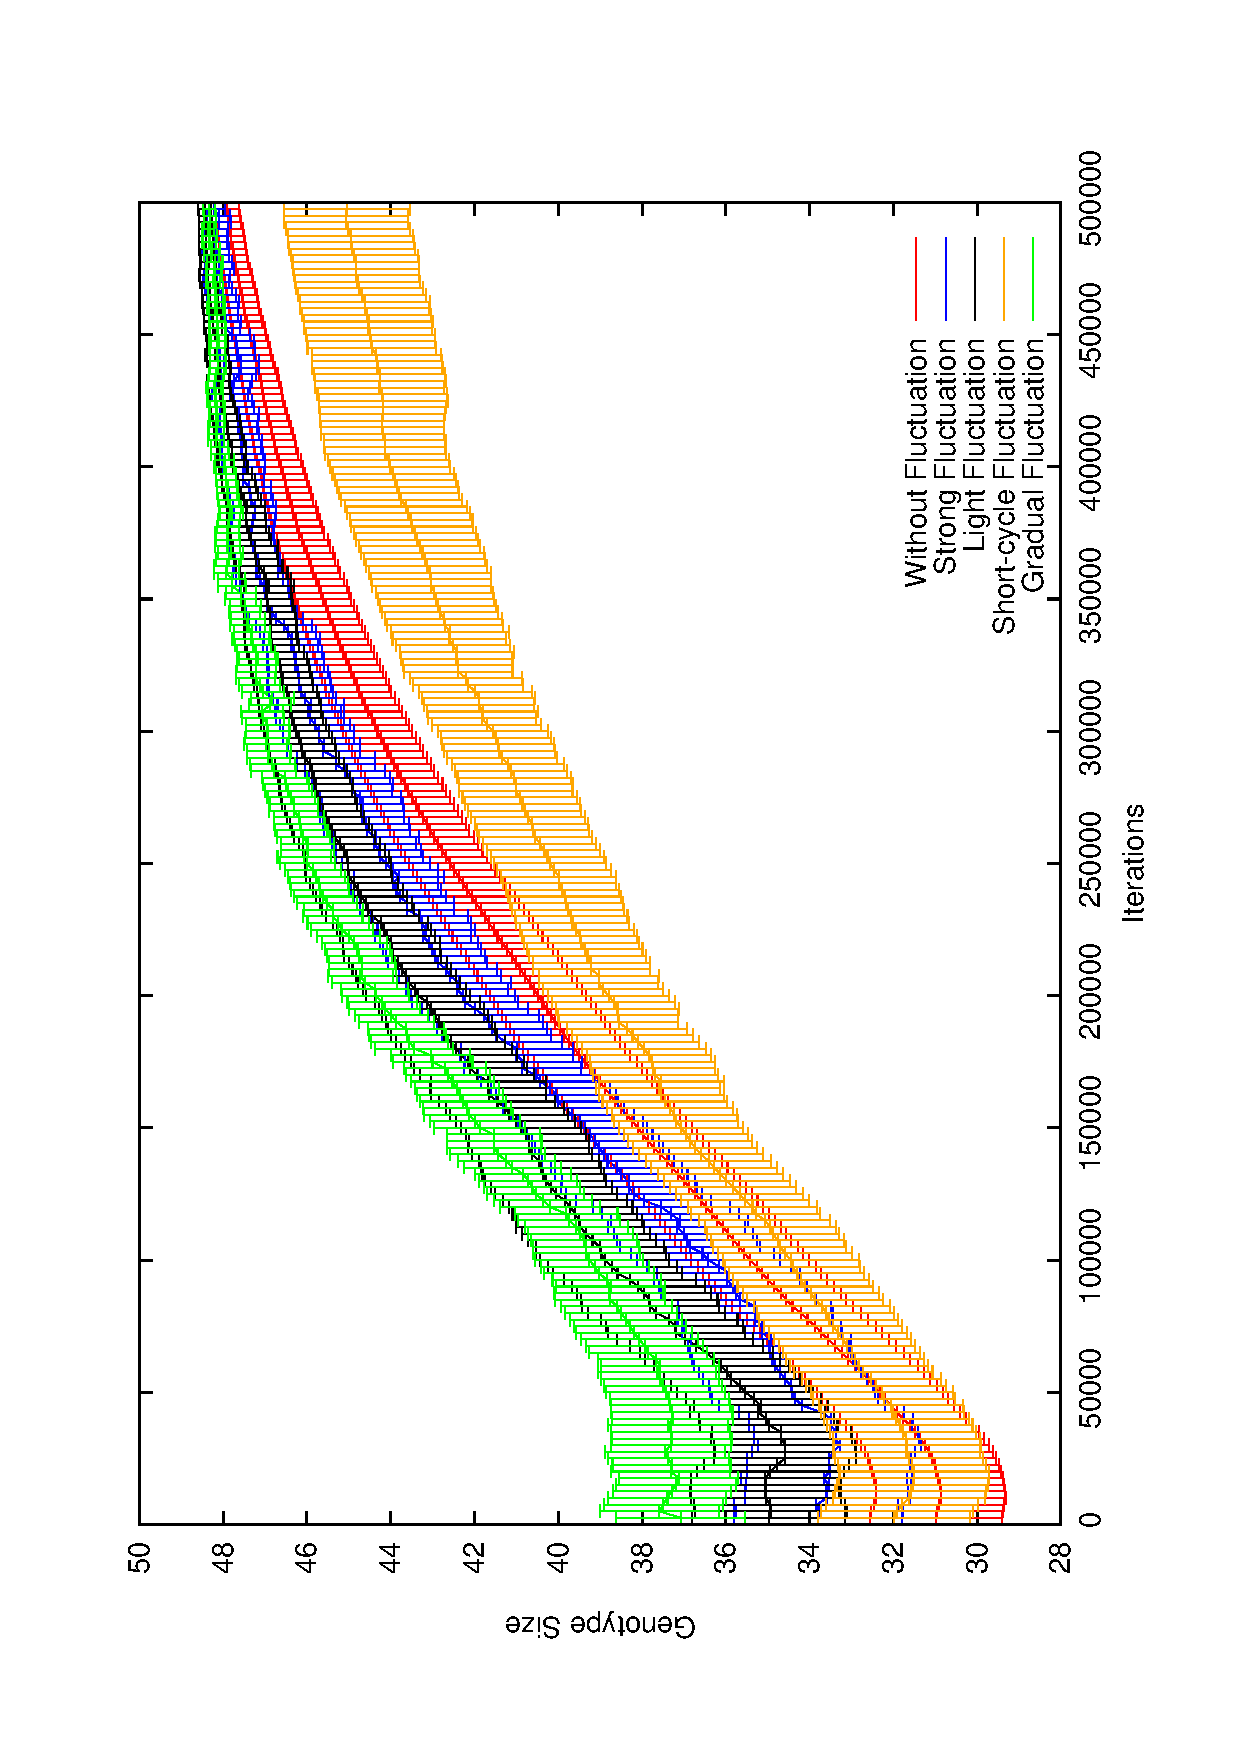
\includegraphics[width=0.7\columnwidth, angle =-90 ]{Size}
\caption{\textbf{Size of genotypes}. 
}
\label{fig:Size}
\end{figure}

\subsection{Size}
Figure~\ref{fig:Size} shows genotype size under the various study conditions. The size is bounded (50 is the maximum size) and it probably limits the differences between those environments as most simulations converge towards this limit, however, one can clearly see here that \emph{Short-cycle Fluctuation} restrict the size of the genotypes while other forms of fluctuations do not appear to have any effect on genotype size..

\begin{figure}[h]
\centering
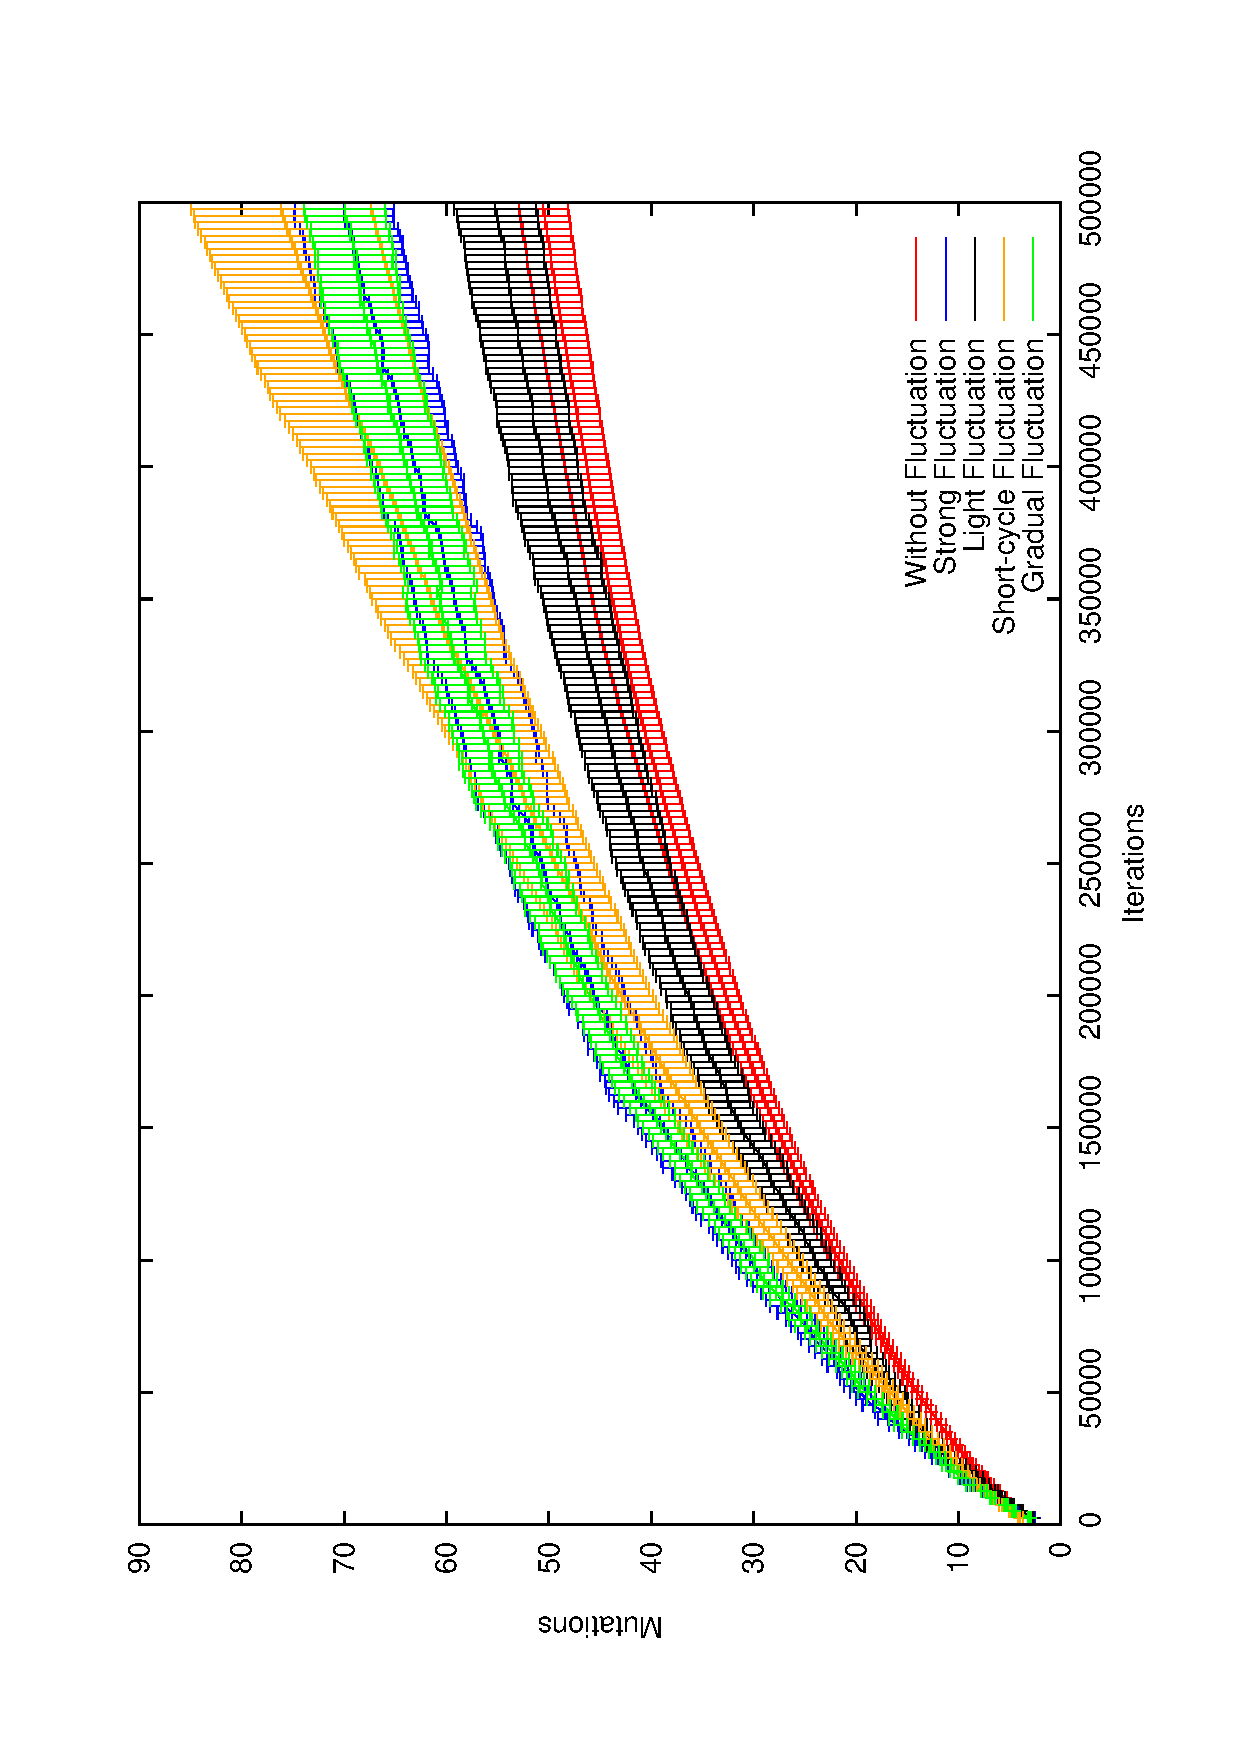
\includegraphics[width=0.7\columnwidth, angle =-90 ]{Mutations}
\caption{\textbf{Mutations of genotypes}.
}
\label{Mutations}
\end{figure}

\begin{figure}[h]
\centering
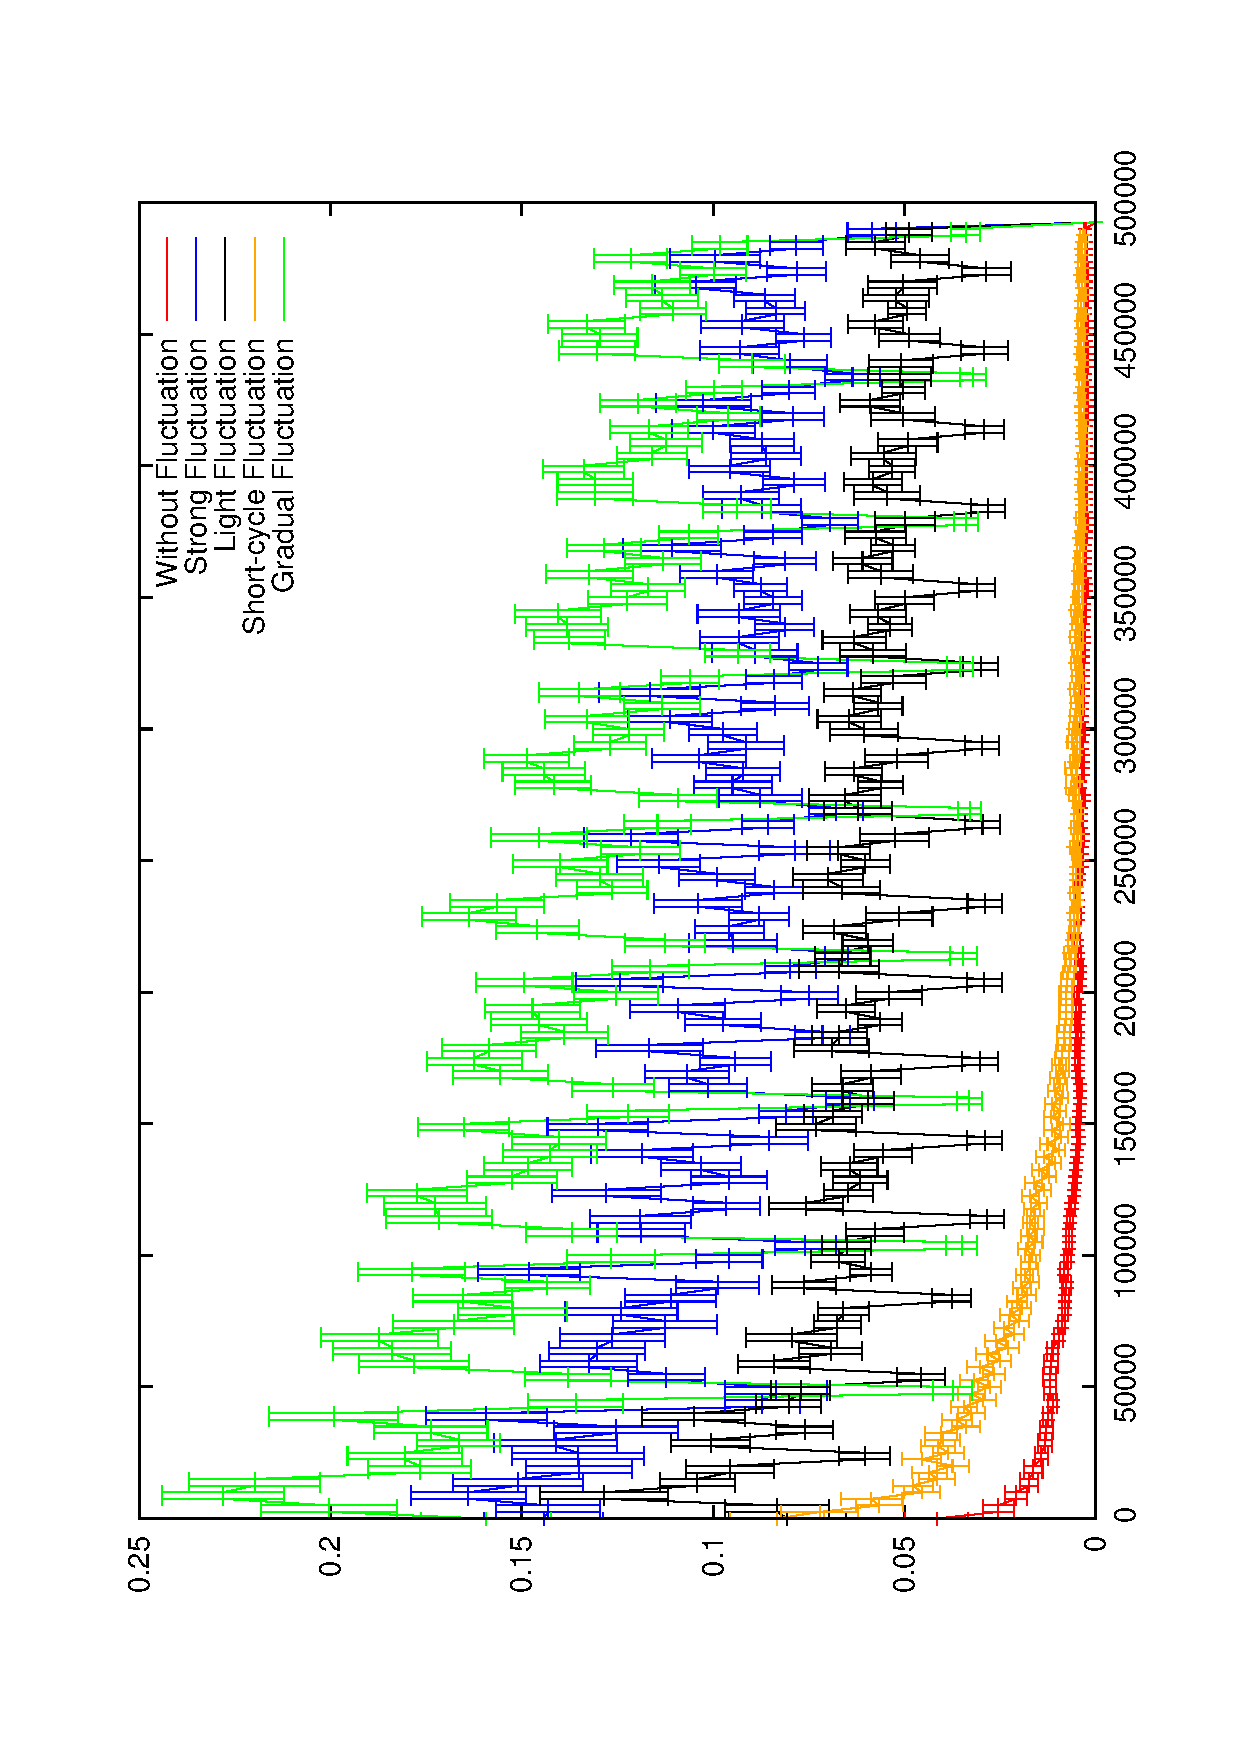
\includegraphics[width=0.7\columnwidth, angle =-90 ]{diffProp}
\caption{\textbf{Changes with following environment} : Here one can see that the impact of environmental fluctuations decreases for \emph{Short-cycle  Fluctuation} while it remains very high for other forms of environmental fluctuations.
}
\label{Mutations}
\end{figure}

\begin{figure}[h]
\centering
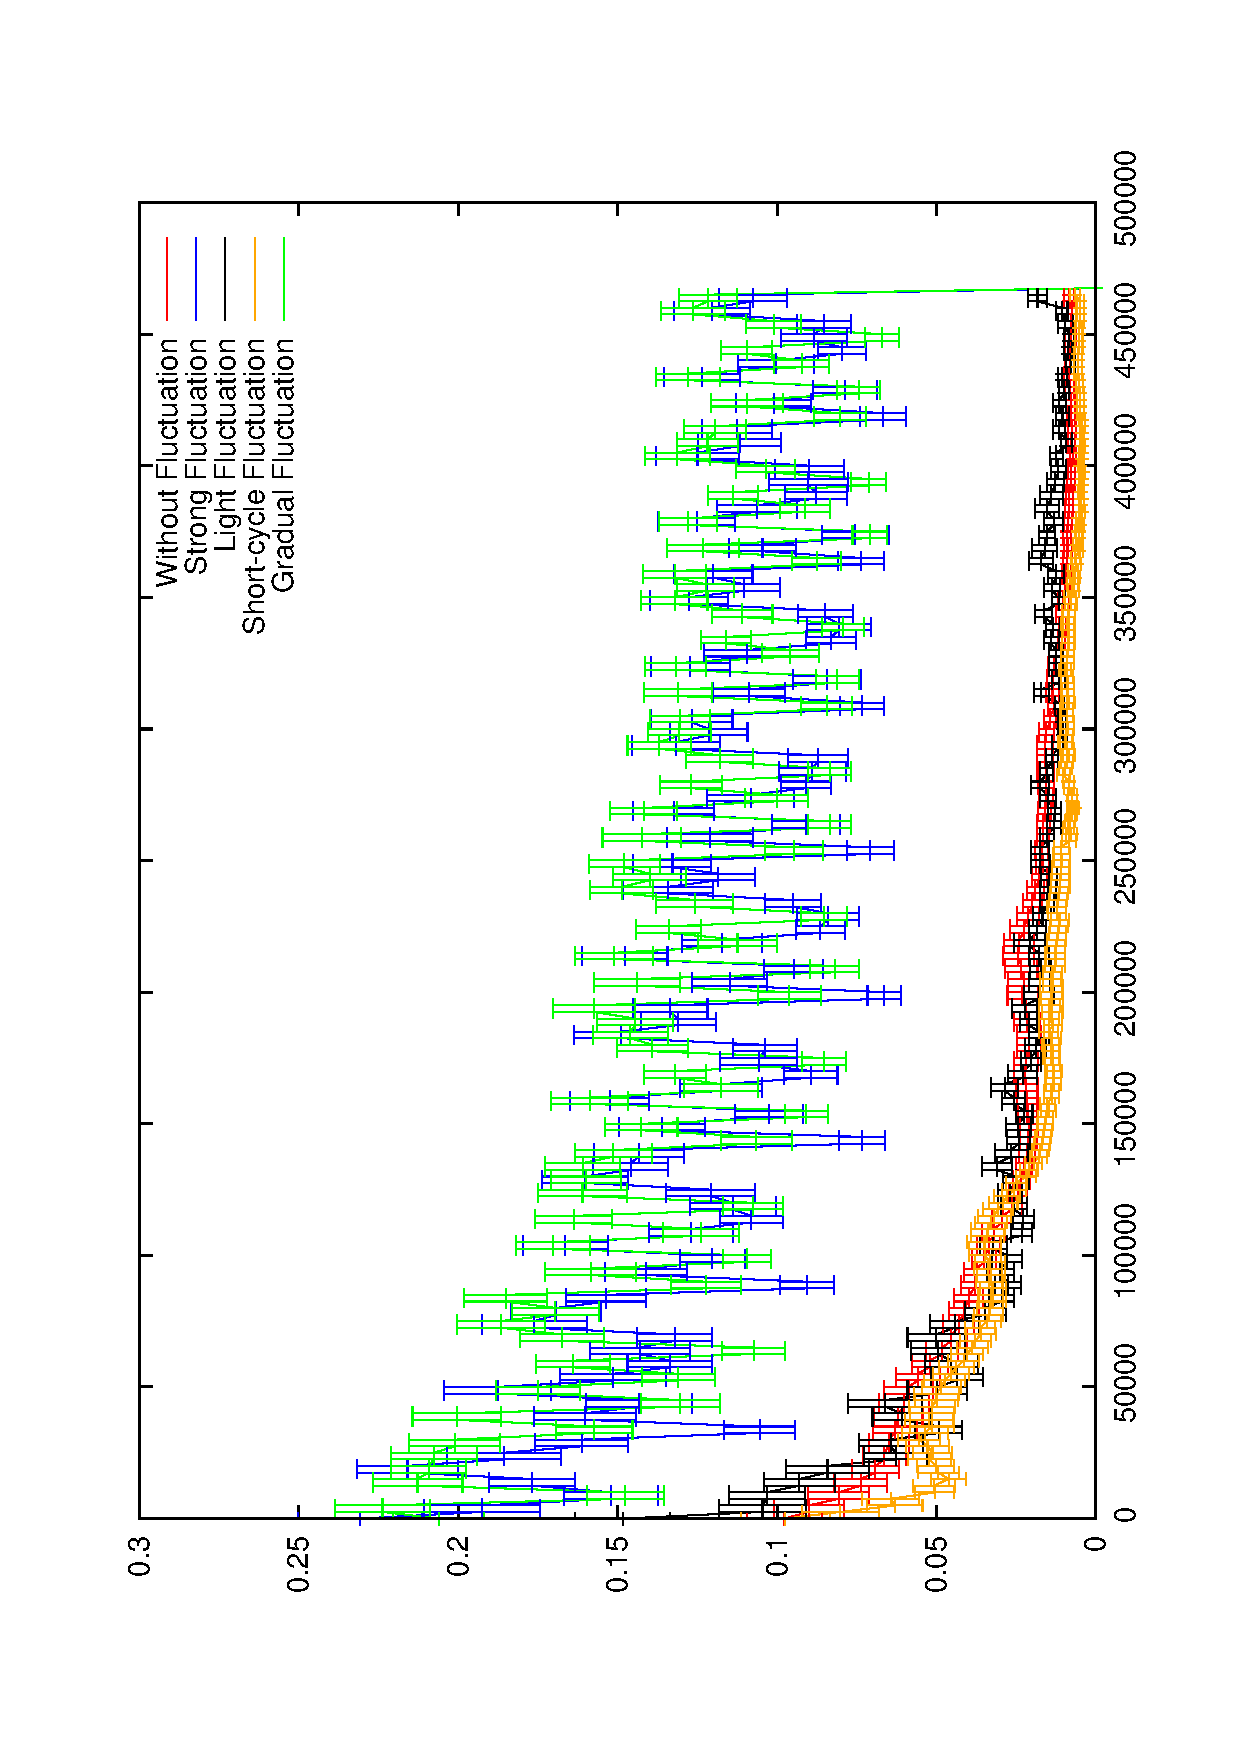
\includegraphics[width=0.7\columnwidth, angle =-90 ]{ProgressProp}
\caption{\textbf{Changes with similar environment} : Here one can see that the impact of environmental fluctuations decreases for \emph{Short-cycle  Fluctuation} and  \emph{Light  Fluctuation}  while it remains very high for other forms of environmental fluctuations.
}
\label{Mutations}
\end{figure}

\begin{figure}[H]
\begin{subfigure}{.25\textwidth}
  \centering
  \includegraphics[width=.7\linewidth, angle =-90]{boxdensitystable.eps}
  \caption{Stable environment.}
  \label{fig:sfig1}
\end{subfigure}%
\begin{subfigure}{.25\textwidth}
  \centering
  \includegraphics[width=.7\linewidth, angle =-90]{boxdensityvariation.eps}
  \caption{Strong Fluctuation.}
  \label{fig:sfig2}
\end{subfigure}

\begin{subfigure}{.25\textwidth}
  \centering
  \includegraphics[width=.7\linewidth, angle =-90]{boxdensityvariationLight.eps}
  \caption{Light Fluctuation.}
  \label{fig:sfig2}
\end{subfigure}%
\begin{subfigure}{.25\textwidth}
  \centering
  \includegraphics[width=.7\linewidth, angle =-90]{boxdensityvariationSmall.eps}
  \caption{Small Fluctuation.}
  \label{fig:sfig1}
\end{subfigure}
\caption{Density of Genotype : Each genotype density is processed in four possible different environments.}
\label{fig:size}
\end{figure}

\begin{figure}[H]
\begin{subfigure}{.25\textwidth}
  \centering
  \includegraphics[width=.7\linewidth, angle =-90]{boxendingsFailedstable.eps}
  \caption{Stable environment.}
  \label{fig:sfig1}
\end{subfigure}%
\begin{subfigure}{.25\textwidth}
  \centering
  \includegraphics[width=.7\linewidth, angle =-90]{boxendingsFailedvariation.eps}
  \caption{Strong Fluctuation.}
  \label{fig:sfig2}
\end{subfigure}

\begin{subfigure}{.25\textwidth}
  \centering
  \includegraphics[width=.7\linewidth, angle =-90]{boxendingsFailedvariationLight.eps}
  \caption{Light Fluctuation.}
  \label{fig:sfig2}
\end{subfigure}%
\begin{subfigure}{.25\textwidth}
  \centering
  \includegraphics[width=.7\linewidth, angle =-90]{boxendingsFailedvariationSmall.eps}
  \caption{Small Fluctuation.}
  \label{fig:sfig1}
\end{subfigure}
\caption{Last iteration with living cells of density runs that didn't reach 60000 iterations. Note that \emph{Short-cycle Fluctuation} genotypes failures are concentrated around iteration 15000 on \emph{Light Fluctuation} density test and around iteration 25000 on \emph{Strong Fluctuation} density test.}
\label{fig:size}
\end{figure}

\section{Discussion}\label{sec:discuss}

\section{Qualitative Analysis}


\section{Conclusions}\label{sec:conc}

\section{Acknowledgement}
The authors gratefully the support of Science Foundation Ireland, grant number:
\bibliography{gp-bibliography,David}{}

\bibliographystyle{plain}
\bibliographystyle{abbrv}
\end{document}
